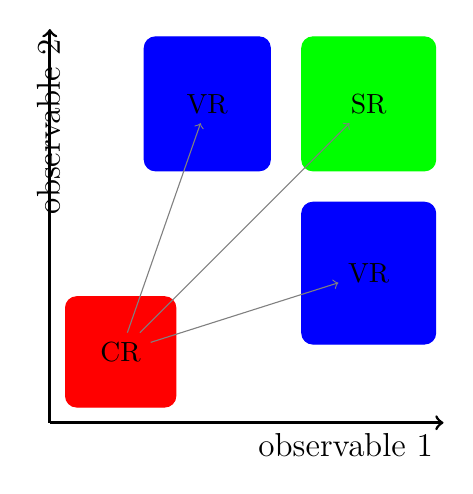
\begin{tikzpicture}

  \tikzstyle{region} = [rounded corners, fill]


  \draw[line width=1, ->] (0,0) -- (5,0) node[below left] {\large observable 1};
  \draw[line width=1, ->] (0,0) -- (0,5) node[left=0.5,rotate=90] {\large observable 2};

  \draw[region, red] (0.2,0.2) rectangle (1.6,1.6) node[midway,black] (CR) {CR};

  \draw[region, green] (3.2,3.2) rectangle (4.9,4.9) node[midway,black] (SR) {SR};

  \draw[region, blue] (3.2,1.0) rectangle (4.9,2.8) node[midway,black] (VR1) {VR};
  \draw[region, blue] (1.2,3.2) rectangle (2.8,4.9) node[midway,black] (VR2) {VR};

  \draw[->,gray] (CR) -- (SR);
  \draw[->,gray] (CR) -- (VR1);
  \draw[->,gray] (CR) -- (VR2);

\end{tikzpicture}
